\documentclass[tikz]{standalone}
\usepackage{amsmath}
\usetikzlibrary{positioning, arrows.meta, calc}

\begin{document}
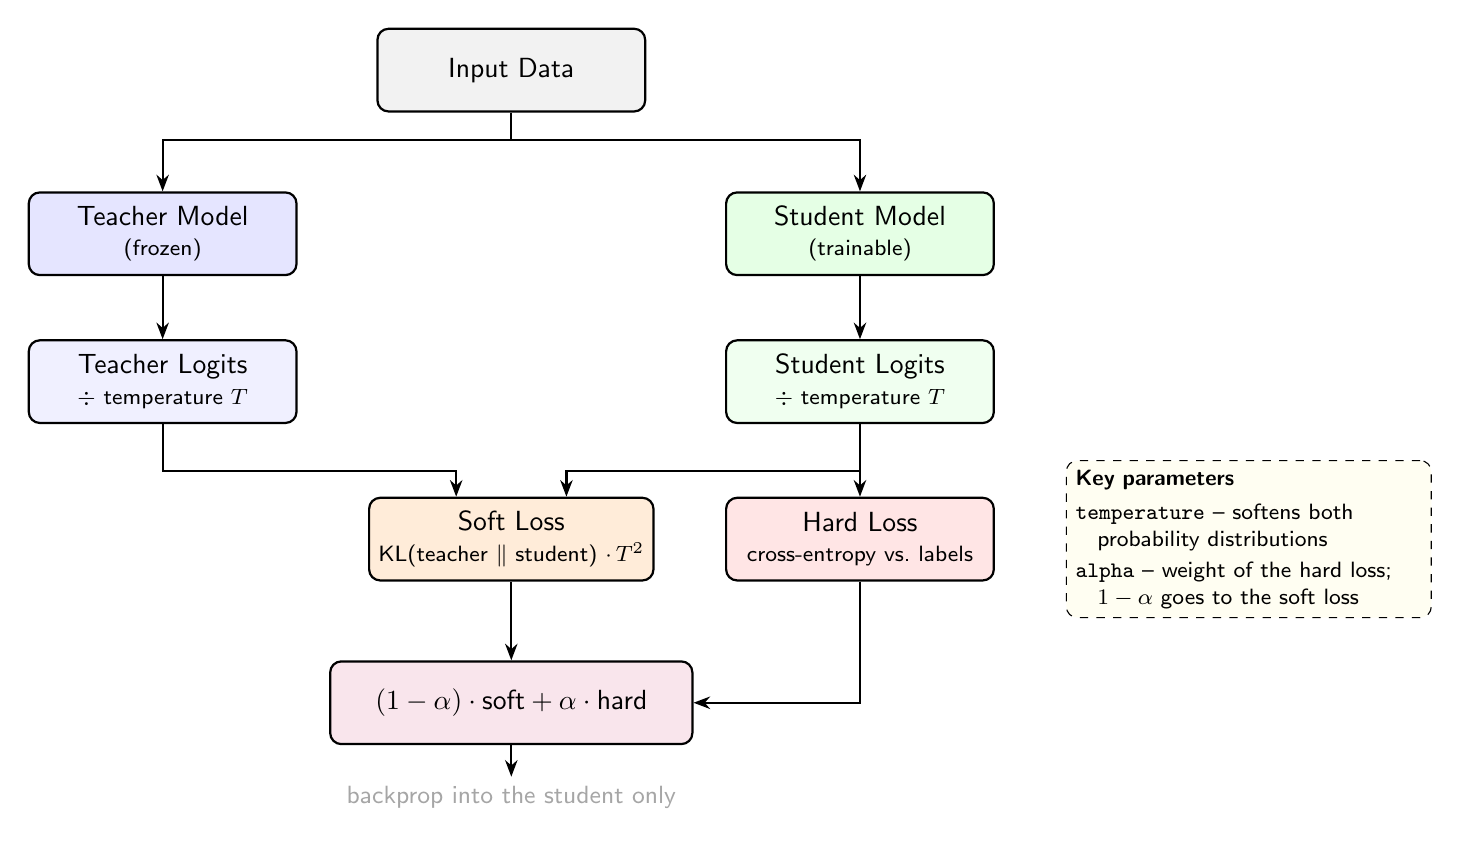
\begin{tikzpicture}[
    every node/.style={font=\sffamily},
    box/.style={draw, thick, rounded corners=4pt, minimum width=3.4cm, minimum height=1.05cm, align=center},
    note/.style={font=\sffamily\small, text=gray!70},
    arr/.style={-{Stealth[length=6pt]}, thick},
]

% ── Models ───────────────────────────────────────────────────────────────────
\node[box, fill=gray!10] (input) {Input Data};
\node[box, fill=blue!10,  below left=1.0cm and 1.0cm of input]  (teacher) {Teacher Model\\[-1pt]{\footnotesize(frozen)}};
\node[box, fill=green!10, below right=1.0cm and 1.0cm of input] (student) {Student Model\\[-1pt]{\footnotesize(trainable)}};

% ── Logits ───────────────────────────────────────────────────────────────────
\node[box, fill=blue!6,  below=0.8cm of teacher] (tlogits) {Teacher Logits\\[-1pt]{\footnotesize$\div$ temperature $T$}};
\node[box, fill=green!6, below=0.8cm of student] (slogits) {Student Logits\\[-1pt]{\footnotesize$\div$ temperature $T$}};

% ── Losses (one row) ─────────────────────────────────────────────────────────
\node[box, fill=orange!15] (soft) at ($(tlogits)!0.5!(slogits) + (0,-2.0cm)$) {Soft Loss\\[-1pt]{\footnotesize KL(teacher $\|$ student) $\cdot\, T^2$}};
\node[box, fill=red!10]    (hard) at (soft -| slogits) {Hard Loss\\[-1pt]{\footnotesize cross-entropy vs.\ labels}};

% ── Weighted sum ─────────────────────────────────────────────────────────────
\node[box, fill=purple!10, minimum width=4.6cm, below=1.0cm of soft] (sum)
      {$(1-\alpha)\cdot\text{soft} + \alpha\cdot\text{hard}$};
\node[note, below=0.4cm of sum] (bp) {backprop into the student only};

% ── Arrows ───────────────────────────────────────────────────────────────────
\draw[arr] (input.south) -- ++(0,-0.35) -| (teacher.north);
\draw[arr] (input.south) -- ++(0,-0.35) -| (student.north);
\draw[arr] (teacher) -- (tlogits);
\draw[arr] (student) -- (slogits);
\draw[arr] (tlogits.south) -- ++(0,-0.6) -| ([xshift=-0.7cm]soft.north);
\draw[arr] (slogits.south) -- ++(0,-0.6) -| ([xshift= 0.7cm]soft.north);
\draw[arr] (slogits) -- (hard);
\draw[arr] (soft) -- (sum);
\draw[arr] (hard.south) |- (sum.east);
\draw[arr] (sum) -- (bp);

% ── Key parameters ───────────────────────────────────────────────────────────
\node[draw, dashed, rounded corners=4pt, fill=yellow!5, text width=4.4cm,
      font=\sffamily\footnotesize, align=left, right=0.9cm of hard] {
    \textbf{Key parameters}\\[3pt]
    \texttt{temperature} -- softens both\\
    \phantom{xx}probability distributions\\[2pt]
    \texttt{alpha} -- weight of the hard loss;\\
    \phantom{xx}$1-\alpha$ goes to the soft loss
};

\end{tikzpicture}
\end{document}
